
\chapter{Figuras, Tabelas e outros elementos}\label{chap:fundamentacaoTeorica}
A seguir ilustra-se a forma de incluir figuras, tabelas, equações, siglas e símbolos no documento, obtendo indexação automática em suas respectivas listas.
A numeração sequencial de figuras, tabelas e equações ocorre de modo automático.
Referências cruzadas são obtidas através dos comandos \verb#\label{}# e \verb#\ref{}#.
Por exemplo, estou me referindo agora a introdução que corresponde ao  capítulo \ref{chap:introducao}. Todos os comandos utilizados para gerar os elementos desse texto estão nos respectivos arquivos dos capítulos. Não os colocaremos aqui para que o texto não fique demasiadamente extenso e não ficarmos repetitivos.

\section{Figuras}
\label{sec:figuras}

Abaixo é apresentado um exemplo de figura. A  figura \ref{fig:brasaouesc} aparece automaticamente na lista de figuras. Para uso avançado de imagens no LATEX, recomenda-se a consulta de literatura especializada.

\begin{figure}[!htb]
	\centering
	\caption{Brasão da UESC}
	
\includegraphics[width=0.3\textwidth]{./04-figuras/brasaouesc}
	\fonte{\citeonline{teste:2014}}
	\label{fig:brasaouesc}
\end{figure}

\subsection{Figuras lado a lado}\label{figladoalado}
Para colocar figuras lado a lado com legendas diferentes utilizamos o pacote {\ttfamily subfigure}, declarado no preâmbulo. Porém o pacote abntex, no qual é baseado a classe, é incompatível com o pacote {\ttfamily subfigure}. Ao tentar usá-lo a compilação apresenta erros de incompatibilidade. 

Para contornar essa situação fiz algumas alterações necessárias no pacote e o renomeei como {\ttfamily subfigureppmgc}. Assim, caso você queira utilizar no seu texto figuras lado a lado com legendas diferentes, deve utilizar essa nova versão do  pacote, o qual se encontra na pasta {\ttfamily pacotes}. A classe já está configurada para utilizá-lo automaticamente.

Caso as figuras que fiquem lado a lado  utilizem apenas uma legenda não há necessidade do pacote, basta chamá-las normalmente no ambiente {\ttfamily figure}.

Abaixo segue um exemplo de como fica a utilização do pacote inserindo figuras lado a lado, com legendas diferentes.\\

\begin{figure}[!htb]
 \caption{Imagens comparando o estado do rio Cachoeira a dez anos atrás e atualmente} \label{fig:estadorc}
\subfigure[ Imagem do rio Cachoeira a dez anos atras\label{fig:rc-adezanos}]{
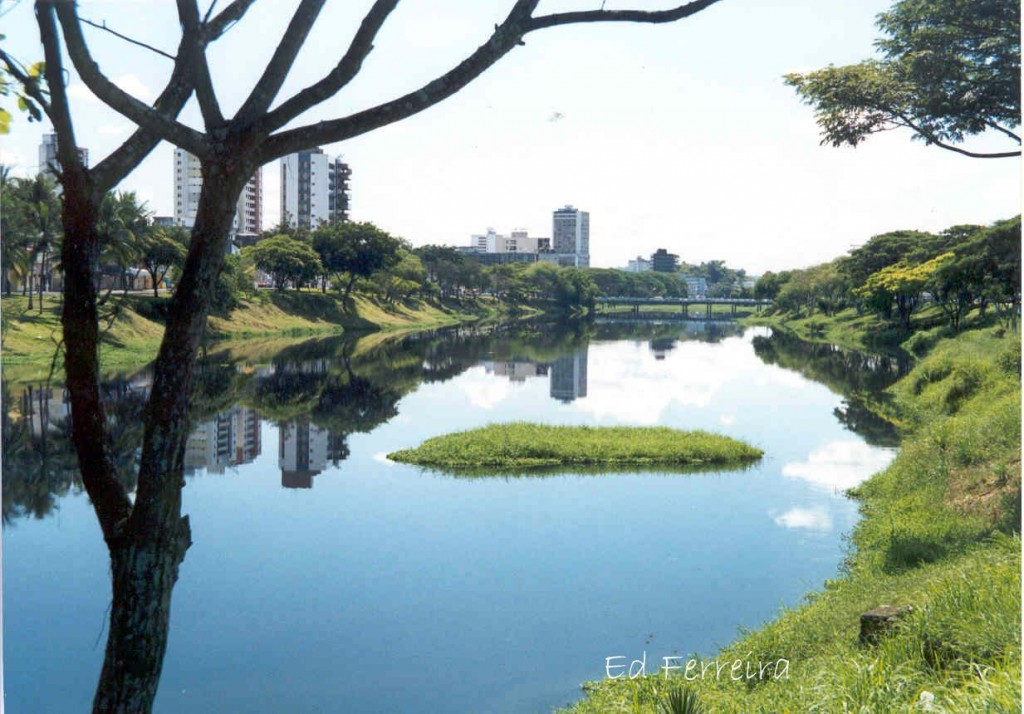
\includegraphics[width=7cm,height=6cm]{04-figuras/rc-adezanos}}
\subfigure[Imagem atual do rio Cachoeira\label{fig:rc-atualmente}]{
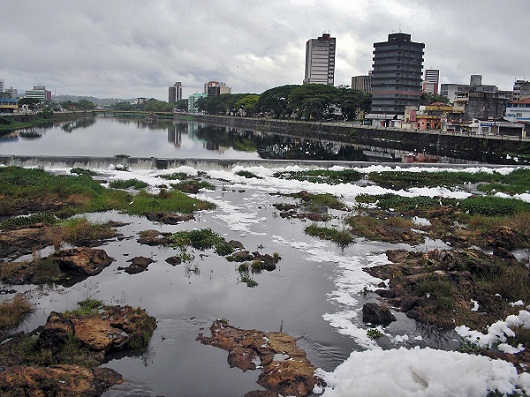
\includegraphics[width=7cm,height=6cm]{04-figuras/rc-atualmente}}
\fonte{Pimenta Blog.BR, no endereço em $<$http://www.pimenta.blog.br/$>$}
\end{figure}
\section{Quadros e Tabelas}
\label{sec:tabelas}

Também é apresentado o exemplo do quadro \ref{qua:comparabd} e da tabela \ref{tab:correlacao}, que aparece automaticamente na lista de quadros e tabelas.
Informações sobre a construção de tabelas no LATEX podem ser encontradas na literatura especializada e diversas apostilas encontradas livremente na internet  \cite{Lamport1986,Buerger1989,reginaldo,camargo}.

\begin{quadro}[!htb]
	\centering
	\caption{Hierarquia de restrições das questões.\label{qua:comparabd}}
	\begin{tabular}{|p{7cm}|p{7cm}|}
		\hline
		\textbf{BD Relacionais} & \textbf{BD Orientados a Objetos} \\
		\hline
		Os dados são passivos, ou seja, certas operações limitadas podem ser automaticamente acionadas quando os dados são usados. Os dados são ativos, ou seja, as solicitações fazem com que os objetos executem seus métodos. & Os processos que usam dados mudam constantemente. \\
		\hline
	\end{tabular}
	\fonte{\citeonline{teste:2014}}
\end{quadro}

\newpage
Exemplos de tabelas:

\begin{table}[!htb]
	\centering
	\caption[Correlação de valores x e y]{Exemplo de uma tabela mostrando a correlação entre x e y.\label{tab:correlacao}}
	\begin{tabular}{cc}
		\hline
			x & y \\
		\hline
			1 & 2 \\
			3 & 4 \\
			5 & 6 \\
			7 & 8 \\
		\hline
	\end{tabular}
	\fonte{Autoria própria.}
\end{table}


\begin{table}[!htb]
	\centering
	\caption[Resultado dos testes]{Resultado dos testes.\label{tab:testes}}
	\begin{tabular}{rrrrr}
		\toprule
			& Valores 1 & Valores 2 & Valores 3 & Valores 4 \\
		\midrule
			Caso 1 & 0,86 & 0,77 & 0,81 & 163 \\
			Caso 2 & 0,19 & 0,74 & 0,25 & 180 \\
			Caso 3 & 1,00 & 1,00 & 1,00 & 170 \\
		\bottomrule
	\end{tabular}
\end{table}


\section{Equações}
\label{sec:equacoes}

A transformada de Laplace é dada na equação \ref{eq:laplace}, enquanto a equação \ref{eq:dft} apresenta a formulação da transformada discreta de Fourier bidimensional\footnote{Deve-se reparar na formatação esteticamente perfeita destas equações.}.

\begin{equation}
	X(s) = \int\limits_{t = -\infty}^{\infty} x(t) \, \text{e}^{-st} \, dt
	\label{eq:laplace}
\end{equation}

\begin{equation}
	F(u, v) = \sum_{m = 0}^{M - 1} \sum_{n = 0}^{N - 1} f(m, n) \exp \left[ -j 2 \pi \left( \frac{u m}{M} + \frac{v n}{N} \right) \right]
	\label{eq:dft}
\end{equation}


